\documentclass[french]{beamer}

\usepackage[utf8]{inputenc}
\usepackage[T1]{fontenc}
\usepackage[english,french]{babel}
\usepackage{graphicx}
\usepackage{amsmath}


\definecolor{darkBlue}{RGB}{20,20,195}

\title{Projet Tétris}
\author{MAILLARD, ROYER, DILLON}
\date{13 mars 2019}


\usetheme{Madrid}
\useinnertheme{circles}
\usecolortheme{whale}


\begin{document}

\AtBeginSection[]{
	\begin{frame}{Plan}
		\tableofcontents[currentsection]
	\end{frame}
}


\begin{frame}

	\begin{columns}

		\hspace{-2.5cm}
		\begin{column}{0.2\textwidth}
			
\includegraphics[scale=0.3]{img/logU.png}
	
		\end{column}
		
		\begin{column}{0.2\textwidth}
			\vspace{0.1cm}
			
\includegraphics[scale=0.045]{img/logF.jpg}

		\end{column}

	\end{columns}

	\vspace{-0.15cm}

	\center{\textsc{\huge \color{darkBlue} Tétris multijoueur}}

	\vspace{-0.5cm}

	\center{\textsc{\color{gray}Soutenance de projet}}

	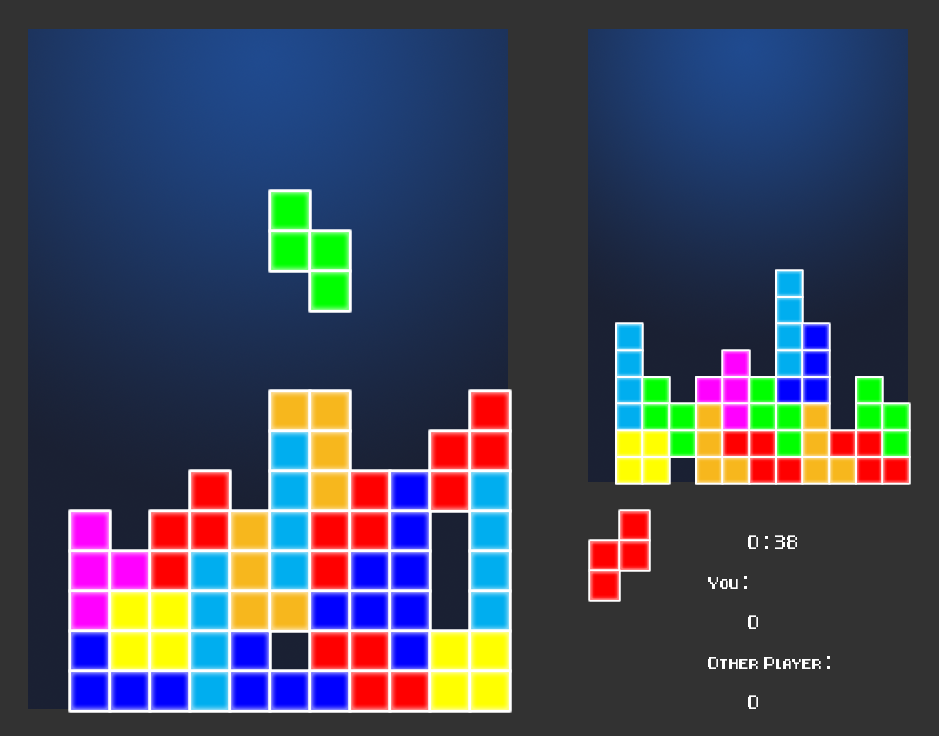
\includegraphics[scale=0.125]{img/vouitris.png}

	\center{\textsc{Cynthia MAILLARD, Félix ROYER, Alexandre DILLON}}
	\vspace{-0.20cm}
	
	\center{\textsc{\large 13 mars 2019}}

	\vspace{0.20cm}

	\textsc{\underline{Tuteur de projet} : \textbf{Julien BERNARD}}

\hspace{2cm}

\end{frame}

\begin{frame}{Plan}

	\tableofcontents

\end{frame}


\section{Adaptation du jeu d'origine}
	\subsection{Le jeu originel}

\begin{frame}{Adaptation du jeu d'origine}{Le jeu originel}
	
	\begin{columns}

		\begin{column}{0.5\textwidth}

			\begin{block}{Le premier Tétris (1984) \\Alekseï Pajitnov}
				\begin{itemize}
					\item jeu de puzzle
					\item réaliser le plus de lignes possibles avec les tétrominos
					\item succès mondial dans les années 1990
					\item adapté sur pratiquement toutes les consoles
				\end{itemize}

			\end{block}

		\end{column}

		\begin{column}{0.4\textwidth}
				\begin{center}
					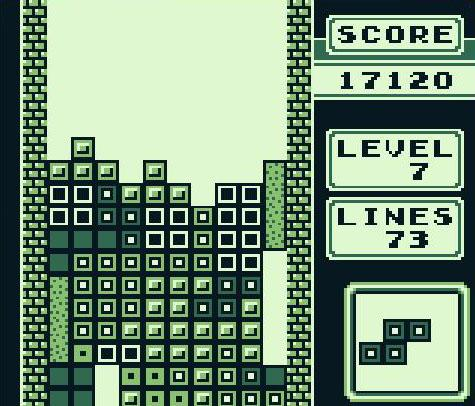
\includegraphics[scale=0.25]{img/Tetris8.jpg}
				\end{center}
		\end{column}

	\end{columns}
\end{frame}

	\subsection{Notre adaptation}

\begin{frame}{Adaptation du jeu d'origine}{Notre adaptation}
	
	\begin{block}{Le cahier des charges}
		\begin{itemize}
			\item client à télécharger et compiler
			\item serveur en ligne
			\item possibilité de redévelopper sa propre interface
			\item chaque joueur joue sur son propre clavier
		\end{itemize}
	\end{block}

\end{frame}

\begin{frame}{Adaptation du jeu d'origine}{Notre adaptation}
	
	\begin{exampleblock}{Les choix d'implémentation}
		\begin{itemize}
			\item le serveur fait loi
			\item le protocole d'échange doit être respecté
			\item détruire des lignes inflige des malus à l'adversaire
		\end{itemize}
	\end{exampleblock}
\end{frame}


\section{Modélisation du jeu}
	\subsection{Architecture réseau}

		\begin{frame}{Modélisation du jeu}{Architecture réseau}
			\begin{center}
				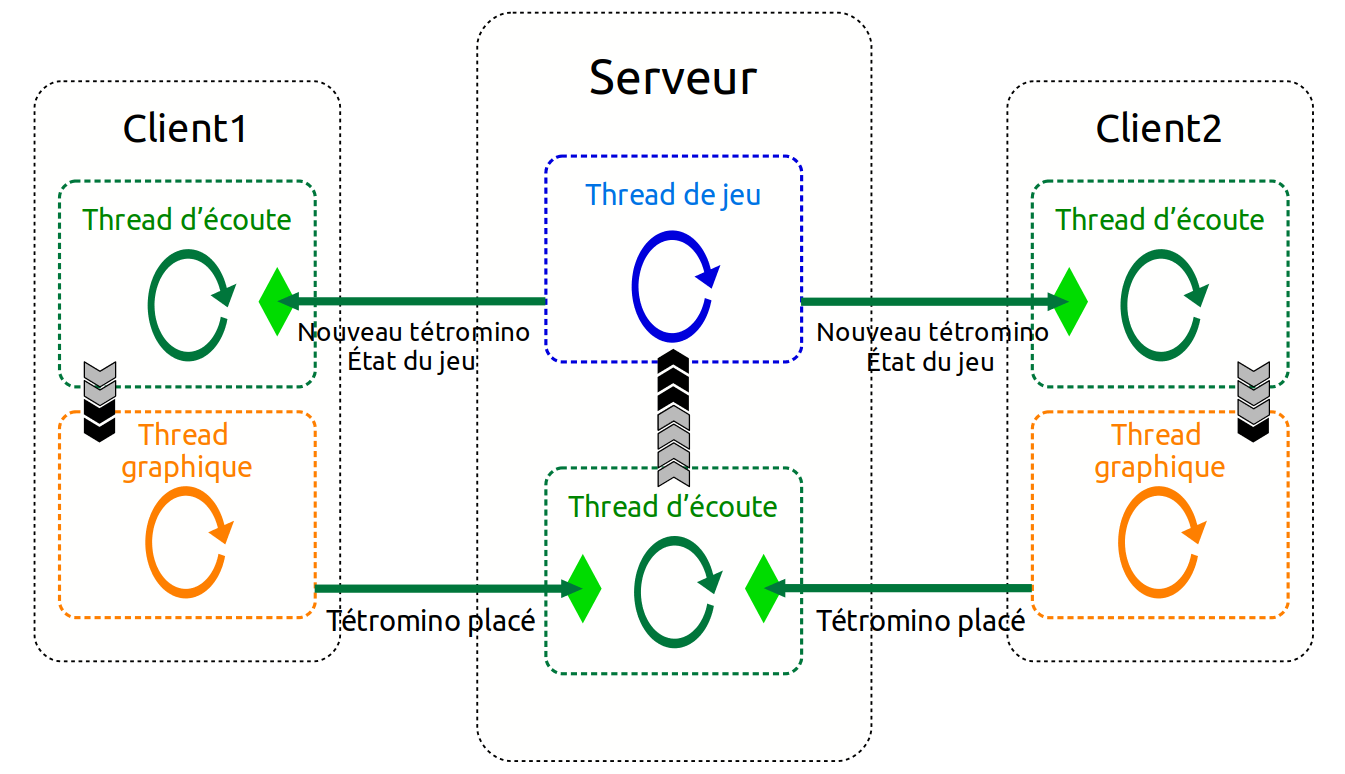
\includegraphics[scale=0.25]{img/archi_reseau.png}
			\end{center}
		\end{frame}

	\subsection{Protocole d'échange de messages}

		\begin{frame}{Modélisation du jeu}{Protocole d'échange de messages}
			\begin{center}
				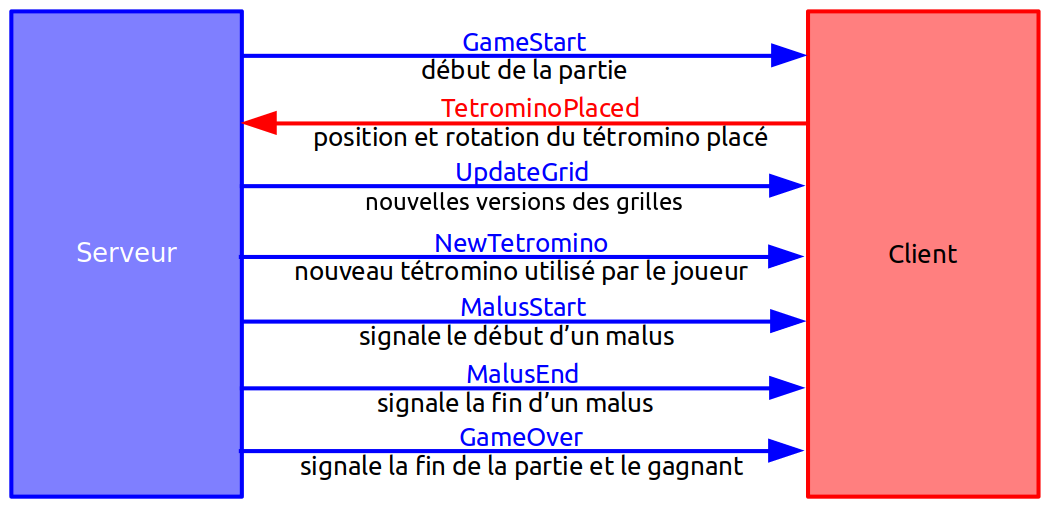
\includegraphics[scale=0.35]{img/ech.png}
			\end{center}
		\end{frame}

\section{Mise en oeuvre}

	\subsection{Le serveur}

	\begin{frame}{Mise en oeuvre}{Le serveur}
		\begin{columns}

			\begin{column}{0.4\textwidth}
				\begin{center}
					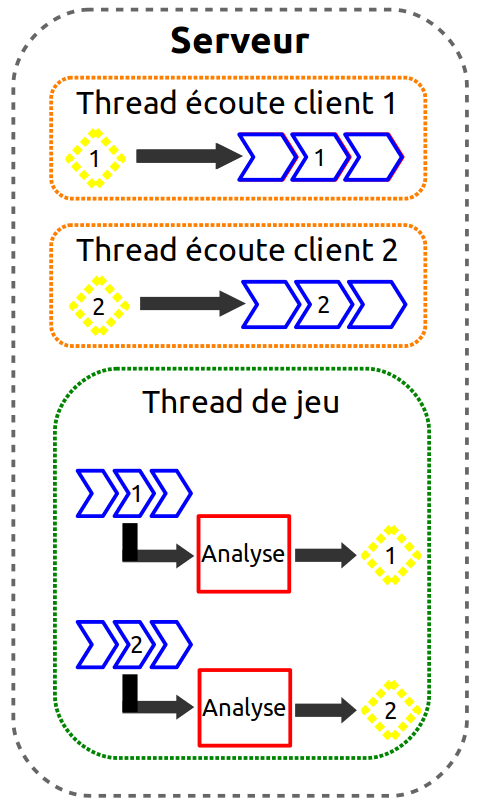
\includegraphics[scale=0.25]{img/serveur.png}
				\end{center}
			\end{column}


			\begin{column}{0.5\textwidth}

				\begin{block}{Les données contenues dans le serveur pour chacun des joueurs}
					\begin{itemize}
						\item grille de jeu
						\item scores
						\item un vérificateur de triche
						\item un gestionnaire de malus
					\end{itemize}

				\end{block}
			\end{column}

		\end{columns}
	\end{frame}




	\begin{frame}[fragile]{Mise en oeuvre}{Le serveur}
		\begin{block}{L'exploitation des messages}
			\begin{verbatim}
			Message(TetrominoPlaced (type, x, y)) :
				VérificationTriche(y)
				MettreAJourGrille(type, x, y) :
					SuppressionLignesPleines()
					MiseAJourScore()

					SI nbLignesSupprimées > 1 :
						EnvoiMalus(autreJoueur, nbLigne)
					FINSI

					EnvoiNouvelleGrilleAuxJoueurs()
			\end{verbatim}
		\end{block}

	\end{frame}



	\begin{frame}{Mise en oeuvre}{Le serveur}
			\begin{columns}

			\begin{column}{0.5\textwidth}
				\begin{block}{Les malus}
					\begin{itemize}
						\item 1 ligne : pas de malus
						\item 2 lignes : empèche la rotation
						\item 3 lignes : accèlération de la chute
						\item 4 lignes : suppression de block en bas du tableau 
					\end{itemize}
				\end{block}
			\end{column}


			\begin{column}{0.3\textwidth}
				
\includegraphics[scale=0.3]{../ressources/malusNoRotate.png}
				
\includegraphics[scale=0.3]{../ressources/malusSpeed.png}
			\end{column}

		\end{columns}


	\end{frame}


	\subsection{La sérialisation}

	\subsection{Les structures de données communes}

	\subsection{Le client graphique}




	
\end{document}